% !TEX root = saveliev_physics_general_course_2.tex
%!TEX TS-program = pdflatex
%!TEX encoding = UTF-8 Unicode


\chapter[INTERFERENCE OF LIGHT]{INTERFERENCE OF LIGHT}\label{chap:17}
\chaptermark{INTERFERENCE OF LIGHT}

\section{Interference of Light Waves}\label{sec:17_1}

Let us assume that two waves of the same frequency, being superposed on each other, produce oscillations of the same direction, namely,
\begin{equation*}
    A_1 \cos(\omega t + \alpha_1),\quad A_2 \cos(\omega t + \alpha_2),
\end{equation*}

\noindent
at a certain point in space.
The amplitude of the resultant oscillation at the given point is determined by the expression
\begin{equation*}
    A^2 = A_1^2 + A_2^2 + 2 A_1 A_2 \cos\delta,
\end{equation*}

\noindent
where $\delta=\alpha_2-\alpha_1$ [see Eq. (7.84) of Vol. I].

If the phase difference $\delta$ of the oscillations set up by the waves remains constant in time, then the waves are called \textbf{coherent}\footnote{We shall discuss the concept of coherence in greater detail in the following.}.

The phase difference $\delta$ for incoherent waves varies continuously and takes on any values with an equal probability.
Hence, the time-averaged value of $\cos\delta$ equals zero.
Therefore,
\begin{equation*}
    \average{A^2} = \average{A_1^2} + \average{A_2^2}.
\end{equation*}

\noindent
Taking into account \eqn{16_10}, we thus conclude that the intensity observed upon the superposition of incoherent waves equals the sum of the intensities produced by each of the waves individually:
\begin{equation}\label{eq:17_1}
    I = I_1 + I_2.
\end{equation}

For coherent waves, $\cos\delta$ has a time-constant value (but a different one for each point of space), so that,
\begin{equation}\label{eq:17_2}
    I = I_1 + I_2 + 2 \sqrt{I_1 I_2} \cos \delta.
\end{equation}

\noindent
At the points of space for which $\cos\delta>0$, the intensity $I$ will exceed $I_1+I_2$; at the points for which $\cos\delta<0$, it will be smaller
than $I_1+I_2$.
Thus, the superposition of coherent light waves is attended by redistribution of the light flux in space.
As a result, maxima of the intensity will appear at some spots and minima at others.
This phenomenon is called the interference of waves.
Interference manifests itself especially clearly when the intensity of both interfering waves is the same: $I_1=I_2$.
Hence, according to \eqn{17_2}, at the maxima $I=4I_1$, while at the minima $I=0$.
For incoherent waves in the same condition, we get the same intensity $I=2I_1$ everywhere [see \eqn{17_1}].

It follows from what has been said above that when a surface is illuminated by several sources of light (for example, by two lamps), an interference pattern ought to be observed with a characteristic alternation of maxima and minima of intensity.
We know from our everyday experience, however, that in this case the illumination of the surface diminishes monotonously with an increasing distance from the light sources, and no interference pattern is observed.
The explanation is that natural light sources are not coherent.

The incoherence of natural light sources is due to the fact that the radiation of a luminous body consists of the waves emitted by many atoms.
The individual atoms emit wave trains with a duration of about \SI{e-8}{\second} and a length of about \SI{3}{\metre} (see \sect{16_1}).
The phase of a new train is not related in any way to that of the preceding one.
In the light wave emitted by a body, the radiation of one group of atoms after about \SI{e-8}{\second} is replaced by the radiation of another group, and the phase of the resultant wave undergoes random changes.

Coherent light waves can be obtained by splitting (by means of reflections or refractions) the wave emitted by a single source into two parts.
If these waves are made to cover different optical paths and are then superposed onto each other, interference is observed.
The difference between the optical paths covered by the interfering waves must not be very great because the oscillations being added must belong to the same resultant wave train.
If this difference will be of the order of one metre, oscillations corresponding to different trains will be superposed, and the phase difference between them will continuously change in a chaotic way.

\begin{figure}[t]
	\begin{center}
		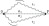
\includegraphics[scale=1]{figures/ch_17/fig_17_1.pdf}
		\caption[]{}
        % \caption[]{Splitting into two coherent waves at point $0$. One wave travels the path $s_1$ in a medium of refractive index $n_1$, and the second wave travels the path $s_2$, in a medium of refractive index $n_2$.}
		\label{fig:17_1}
	\end{center}
	\vspace{-0.8cm}
\end{figure}

Assume that the splitting into two coherent waves occurs at point $0$ (\fig{17_1}).
Up to point P, the first wave travels the path $s_1$ in a medium of refractive index $n_1$, and the second wave travels the path $s_2$, in a medium of refractive index $n_2$.
If the phase of oscillations at point $0$ is $\omega t$, then the first wave will produce the oscillation $A_1\cos\omega(t-s_1/v_1)$ at point P, and the second wave, the oscillation $A_2\cos\omega(t-s_2/v_2)$ at this point; $v_1=c/n_1$ and $v_2=c/n_2$ are the phase velocities of the waves.
Hence, the difference between the phases of the oscillations produced by the waves at point P will be
\begin{equation*}
    \delta = \omega \parenthesis{\frac{s_2}{v_2} - \frac{s_1}{v_1}} = \frac{\omega}{c} (n_2 s_2 - n_1 s_1).
\end{equation*}

\noindent
Replacing $\omega/c$ with $2\pi\nu/c = 2\pi/\lambda_0$ (where $\lambda_0$ is the wavelength in
a vacuum), the expression for the phase difference can be written in the form
\begin{equation}\label{eq:17_3}
    \delta = \frac{2 \pi}{\lambda_0} \Delta,
\end{equation}

\noindent
where
\begin{equation}\label{eq:17_4}
    \Delta = n_2 s_2 - n_1 s_1 = L_1 - L_2,
\end{equation}

\noindent
is a quantity equal to the difference between the optical paths travelled by the waves and is called the \textbf{difference in optical path} [compare with \eqn{16_55}].

A glance at \eqn{17_3} shows that if the difference in the optical path equals an integral number of wavelengths in a vacuum:
\begin{equation}\label{eq:17_5}
    \Delta = \pm m \lambda_0 \quad (m = 0, 1, 2, \ldots),
\end{equation}

\noindent
then the phase difference $\delta$ is a multiple of $2\pi$, and the oscillations produced at point P by both waves will occur with the same phase.
Thus, \eqn{17_5} is the condition for an interference maximum, \ie, for \textbf{constructive interference}.

If $\Delta$ equals a half-integral number of wavelengths in a vacuum:
\begin{equation}\label{eq:17_6}
    \Delta = \pm \parenthesis{m + \frac{1}{2}} \lambda_0 \quad (m = 0, 1, 2, \ldots),
\end{equation}

\noindent
then, $\delta=\pm(2m + 1)\pi$, so that the oscillations at point P are in counterphase.
Thus, \eqn{17_6} is the condition for an interference minimum, \ie, for \textbf{destructive interference}.

Let us consider two cylindrical coherent light waves emerging from sources S$_1$ and S$_2$ having the form of parallel thin luminous filaments or narrow slits (\fig{17_2}).
The region in which these waves overlap is called the \textbf{interference field}.
Within this entire region, there are observed alternating places with maximum and minimum intensity of light.
If we introduce a screen into the interference field, we shall see on it an interference pattern having the form of alternating light and dark fringes.
Let us calculate the width of these fringes, assuming that the screen is parallel to a plane passing through sources S$_1$ and S$_2$.
We shall characterize the position of a point on the screen by the coordinate x measured in a direction at right angles to lines S$_1$ and S$_2$.
We shall choose the beginning of our readings at point $0$ relative to which S$_1$ and S$_2$ are arranged symmetrically.
We shall consider that the sources oscillate in the same phase.
Examination of \fig{17_2} shows that
\begin{equation*}
    s_1^2 = l^2 + \parenthesis{x - \frac{d}{2}}^2,\quad s_2^2 = l^2 + \parenthesis{x + \frac{d}{2}}^2.
\end{equation*}

\begin{figure}[t]
	\begin{center}
		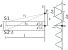
\includegraphics[scale=0.95]{figures/ch_17/fig_17_2.pdf}
		\caption[]{}
        % \caption[]{Interference field of two cylindrical coherent light waves emerging from sources S$_1$ and S$_2$ having the form of parallel thin luminous filaments or narrow slits.}
		\label{fig:17_2}
	\end{center}
	\vspace{-0.9cm}
\end{figure}

\noindent
Hence,
\begin{equation*}
    s_2^2 - s_1^2 = (s_2 + s_1) (s_2 - s_1) = 2xd.
\end{equation*}

It will be established somewhat later that to obtain a distinguishable interference pattern, the distance between the sources $d$ must be considerably smaller than the distance to the screen $l$.
The distance $x$ within whose limits interference fringes are formed is also considerably smaller than $l$.
In these conditions, we can assume that $s_2+s_1 \approx 2l$.
Thus, $s_2-s_1=xd/l$.
Multiplying $s_2-s_1$ by the refractive index of the medium $n$, we get the difference in the optical path
\begin{equation}\label{eq:17_7}
    \Delta = n \frac{xd}{l}.
\end{equation}

\noindent
The introduction of this value of $\Delta$ into condition \eqref{eq:17_5} shows that intensity maxima will be observed at values of $x$ equal to
\begin{equation}\label{eq:17_8}
    \ab{x}{max} = \pm m \frac{l}{d} \lambda \quad (m = 0, 1, 2, \ldots).
\end{equation}

\noindent
Here $\lambda=\lambda_0/n$ is the wavelength in the medium filling the space between the sources and the screen.

Using the value of $\Delta$ given by \eqn{17_7} in condition \eqref{eq:17_6}, we get the coordinates of the intensity minima:
\begin{equation}\label{eq:17_9}
    \ab{x}{min} = \pm \parenthesis{m + \frac{1}{2}} \frac{l}{d} \lambda \quad (m = 0, 1, 2, \ldots).
\end{equation}

Let us call the distance between two adjacent intensity maxima the \textbf{distance between interference fringes}, and the distance between
adjacent intensity minima the \textbf{width of an interference fringe}.
It can be seen from \eqns{17_8}{17_9} that the distance between fringes and the width of a fringe have the same value equal to
\begin{equation}\label{eq:17_10}
    \Delta{x} = \frac{l}{d} \lambda.
\end{equation}

According to \eqn{17_10}, the distance between the fringes grows with a decreasing distance $d$ between the sources.
If $d$ were comparable with $l$, the distance between the fringes would be of the same order as $\lambda$, \ie, would be several scores of micrometres.
In this case, the separate fringes would be absolutely indistinguishable.
For an interference pattern to become distinct, the above-mentioned condition $d\ll l$ must be observed.

If the intensity of the interfering waves is the same ($I_1=I_2=I_0$), then according to \eqn{17_2} the resultant intensity at the points
for which the phase difference is $\delta$ is determined by the expression
\begin{equation*}
    I = 2 I_0 (1 + \cos\delta) = 4 I_0 \cos^2\parenthesis{\frac{\delta}{2}}.
\end{equation*}

\noindent
Since $\delta$ is proportional to $\Delta$ [see \eqn{17_3}], then, in accordance with \eqn{17_7}, $\delta$ grows proportionally to $x$.
Hence, the intensity varies along the screen in accordance with the law of cosine square.
The right-hand part of \fig{17_2} shows the dependence of $I$ on $x$ obtained in monochromatic light.

The width of the interference fringes and their spacing depend on the wavelength $\lambda$.
The maxima of all wavelengths will coincide only at the centre of a pattern when $x=0$.
With an increasing distance from the centre of the pattern, the maxima of different colours become displaced from one another more and more.
The result is blurring of the interference pattern when it is observed in white light.
The number of distinguishable interference fringes appreciably grows in monochromatic light.

Having measured the distance between the fringes $\Delta{x}$ and knowing $l$ and $d$, we can use \eqn{17_10} to find $\lambda$.
It is exactly from experiments involving the interference of light that the wavelengths for light rays of various colours were determined for the first time.

We have considered the interference of two cylindrical waves.
Let us see what happens when two plane waves are superposed.
Assume that the amplitudes of these waves are the same, and the directions of their propagation make the angle $2\varphi$ (\fig{17_3}).
We shall consider that the directions of oscillations of the light vector are perpendicular to the plane of the drawing.
The wave vectors $\vec{k}_1$ and $\vec{k}_2$ are in the plane of the drawing and have the same magnitude equal to $k=2\pi/\lambda$.
Let us write the equations of these waves:
\begin{align*}
    A \cos(\omega t - \vec{k}_1\ccdot\vec{r}) & = A \cos(\omega t - k \sin\varphi \times x - k \cos\varphi \times y),\\
    A \cos(\omega t - \vec{k}_2\ccdot\vec{r}) & = A \cos(\omega t + k \sin\varphi \times x - k \cos\varphi \times y).
\end{align*}

\begin{figure}[t]
	\begin{center}
		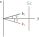
\includegraphics[scale=1]{figures/ch_17/fig_17_3.pdf}
		\caption[]{}
        % \caption[]{Superposition of two plane waves with the same amplitudes, and the directions of their propagation making the angle $2\varphi$.}
		\label{fig:17_3}
	\end{center}
	\vspace{-0.9cm}
\end{figure}

The resultant oscillation at points with the coordinates $x$ and $y$ has the form
\begin{align}
    A \cos(\omega t - k \sin\varphi \times x &- k \cos\varphi \times y) + A \cos(\omega t + k \sin\varphi \times x - k \cos\varphi \times y)\nonumber\\
    & = 2A \cos(k \sin\varphi \times x) \cos(\omega t - k \cos\varphi \times y). \label{eq:17_11}
\end{align}

It follows from this equation that at points where $k \sin\varphi \times x = \pm m\pi (m = 0, 1, 2, \ldots)$, the amplitude of the oscillations
is $2A$; where $k \sin\varphi \times x = \pm (m+1/2)\pi$, the amplitude of the oscillations
is zero.
No matter where we place screen Sc, which is perpendicular to the $y$-axis, we shall observe on it a system of alternating light and dark fringes parallel to the $z$-axis (this axis is perpendicular to the plane of the drawing).
The coordinates of the intensity maxima will be
\begin{equation}\label{eq:17_12}
    \ab{x}{max} = \pm \frac{m \pi}{k \sin\varphi} = \pm \frac{m \lambda}{2 \sin\varphi}.
\end{equation}

Only the phase of the oscillations depends on the position of the screen (on the coordinate $y$) [see \eqn{17_11}].

We have assumed for simplicity that the initial phases of interfering waves are zero.
If the difference between these phases is other than zero, a constant addend will appear in \eqn{17_12}---the fringe pattern will move along the screen.

\section{Coherence}\label{sec:17_2}

By \textbf{coherence} is meant the coordinated proceeding of several oscillatory or wave processes.
The degree of coordination may vary.
We can accordingly introduce the concept of the \textbf{degree of coherence} of two waves.

\textbf{Temporal} and \textbf{spatial coherence} are distinguished.
We shall begin with a discussion of temporal coherence.

\textbf{Temporal Coherence.}
The process of interference described in the preceding section is idealized.
This process is actually much more complicated.
The reason is that a monochromatic wave described
by the expression
\begin{equation*}
    A \cos(\omega t - kr + \alpha),
\end{equation*}

\noindent
where $A$, $\omega$, and $\alpha$ are constants, is an abstraction.
A real light wave is formed by the superposition of oscillations of all possible frequencies (or wavelengths) confined within a more or less narrow but finite range of frequencies $\Delta{\omega}$ (or the corresponding range of wavelengths $\Delta{\lambda}$).
Even for light considered to be monochromatic (single-coloured), the frequency interval $\Delta{\omega}$ is finite\footnote{The spectral lines emitted by atoms have a ``natural'' width of the order of \SI{e-8}{\radian\per\second} ($\Delta{\lambda}\sim\SI{e-4}{\angstrom}$).}.
In addition, the amplitude of the wave $A$ and the phase $\alpha$ undergo continuous random (chaotic) changes with time.
Hence, the oscillations produced at a certain point of space by two superposed light waves have the form
\begin{equation}\label{eq:17_13}
    A_1(t) \cos[\omega_1(t) t + \alpha_1(t)],\quad A_2(t) \cos[\omega_2(t) t + \alpha_2(t)],
\end{equation}

\noindent
the chaotic changes in the functions $A_1(t)$, $\omega_1(t)$, $\alpha_1(t)$, $A_2(t)$, $\omega_2(t)$, and $\alpha_2(t)$ being absolutely independent.

We shall assume for simplicity's sake that the amplitudes $A_1$ and $A_2$ are constant.
Changes in the frequency and phase can be re duced either to a change only in the phase, or to a change only in the frequency.
Let us write the function
\begin{equation}\label{eq:17_14}
    f(t) = A \cos[\omega(t) t + \alpha(t)],
\end{equation}

\noindent
in the form
\begin{equation*}
    f(t) = A \cos\{\omega_0 t + [\omega(t) - \omega_0] t + \alpha(t)\},
\end{equation*}

\noindent
where $\omega_0$ is a certain average value of the frequency, and introduce the notation $[\omega(t) - \omega_0] t + \alpha(t) = \alpha'(t)$.
Equation \eqref{eq:17_14} will, thus, become
\begin{equation}\label{eq:17_15}
    f(t) = A \cos[\omega_0 t + \alpha'(t)].
\end{equation}

\noindent
We have obtained a function in which only the phase of the oscillation changes chaotically.

On the other hand, it is proved in mathematics that an inharmonic function, for example, function \eqref{eq:17_14}, can be represented in the form of the sum of harmonic functions with frequencies confined within a certain interval $\Delta(\omega)$ [see \eqn{17_16}].

Thus, when considering the matter of coherence, two approaches are possible: a ``phase'' one and a ``frequency'' one.
Let us begin with the phase approach.
Assume that the frequencies $\omega_1$ and $\omega_2$ in Eqs. \eqref{eq:17_13} satisfy the condition $\omega_1 = \omega_2 = \text{constant}$.
Now let us find the influence of a change in the phases $\alpha_1$ and $\alpha_2$.
According to \eqn{17_12}, with our assumptions, the intensity of light at a given point is determined by the expression
\begin{equation*}
    I = I_1 + I_2 + 2 \sqrt{I_1 I_2} \cos[\delta(t)],
\end{equation*}

\noindent
where $\delta(t) = \alpha_2(t) - \alpha_1(t)$.
The last addend in this equation is called the \textbf{interference term}.

An instrument that can be used to observe an interference pattern (the eye\footnote{We remind our reader that the showing of motion picture films is based on the inertia of visual perception, which is about \SI{0.1}{\second}.}, a photographic plate, etc.) has a certain inertia.
In this connection, it registers a pattern averaged over the time interval $\ab{t}{instr}$ needed for ``operation'' of the instrument.
If during the time $\ab{t}{instr}$ the factor $\cos[\delta(t)]$ takes on all the values from $-1$ to $+1$, the average value of the interference term will be zero.
Therefore, the intensity registered by the instrument will equal the sum of the intensities produced at a given point by each of the waves separately---interference is absent, and we are forced to acknowledge that the waves are incoherent.

If during the time $\ab{t}{instr}$, however, the value of $\cos[\delta(t)]$ remains virtually constant\footnote{The phase difference $\delta(t)$ varies for different points of space. The influence of the interference term manifests itself at the points where it differs from zero.}, the instrument will detect interference, and the waves must be acknowledged as coherent.

It follows from the above that the concept of coherence is relative: two waves can behave like coherent ones when observed using one instrument (having a low inertia), and like incoherent ones when observed using another instrument (having a high inertia).
The coherent properties of waves are characterized by introducing the \textbf{coherence time} $\ab{t}{coh}$.
It is defined as the time during which a chance change in the wave phase $\alpha(t)$ reaches a value of the order of $\pi$.
During the time $\ab{t}{coh}$, an oscillation, as it were, forgets its initial phase and becomes incoherent with respect to itself.

Using the concept of the coherence time, we can say that when the instrument time is much greater than the coherence time of the superposed waves ($\ab{t}{instr}\gg\ab{t}{coh}$), the instrument does not register interference.
When $\ab{t}{instr}\ll\ab{t}{coh}$, the instrument will detect a sharp interference pattern.
At intermediate values of $\ab{t}{instr}$, the sharpness of the pattern will diminish as $\ab{t}{instr}$ grows from values smaller than
$\ab{t}{coh}$ to values greater than it.

The distance $\ab{l}{coh} = c\ab{t}{coh}$ over which a wave travels during the time $\ab{l}{coh}$ is called the \textbf{coherence length} (or the \textbf{train length}).
The coherence length is the distance over which a chance change in the phase reaches a value of about $\pi$.
To obtain an interference pattern by splitting a natural wave into two parts, it is essential that the optical path difference $\Delta$ be smaller than the coherence length.
This requirement limits the number of visible interference fringes observed when using the layout shown in \fig{17_2}.
An increase in the fringe number $m$ is attended by a growth in the path difference.
As a result, the sharpness of the fringes becomes poorer and poorer.

Let us pass over to a consideration of the part of the non-monochromatic nature of light waves.
Assume that light consists of a sequence of identical trains of frequency $\omega_0$ and duration $T$.
When one train is replaced with another one, the phase experiences disordered changes.
As a result, the trains are mutually incoherent.
With these assumptions, the duration of a train $\tau$ virtually coincides with the coherence
time $\ab{t}{coh}$.

In mathematics, the Fourier theorem is proved, according to which any finite and integrable function $F(t)$ can be represented in the form of the sum of an infinite number of harmonic components with a continuously changing frequency:
\begin{equation}\label{eq:17_16}
    F(t) = \int_{-\infty}{+\infty} A(\omega) \, e^{i\omega t}\, \deriv{\omega}.
\end{equation}

\noindent
Expression \eqref{eq:17_16} is known as the \textbf{Fourier integral}.
The function $A(\omega)$ inside the integral is the amplitude of the relevant monochromatic component.
According to the theory of Fourier integrals, the analytical form of the function $A(\omega)$ is determined by the expression
\begin{equation}\label{eq:17_17}
    A(\omega) = 2\pi \int_{-\infty}^{+\infty} F(\xi)\, e^{-i\omega \xi}\, \deriv{\xi},
\end{equation}

\noindent
where $\xi$ is an auxiliary integration variable.

Assume that the function $F(t)$ describes a light disturbance at a certain point at the moment of time $t$ due to a single wave train.
Hence, it is determined by the conditions
\begin{align*}
    F(t) &= A_0\, \exp(i \omega_0 t) \quad \text{at } |t| \ll \frac{\tau}{2} \\
    F(t) &= 0 \quad\quad\quad\quad\quad\quad\! \text{at } |t| > \frac{\tau}{2}.
\end{align*}

\noindent
A graph of the real part of this function is given in \fig{17_4}.

\begin{figure}[t]
	\begin{center}
		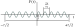
\includegraphics[scale=1]{figures/ch_17/fig_17_4.pdf}
		\caption[]{}
        % \caption[]{Real part of function $F(t)$.}
		\label{fig:17_4}
	\end{center}
	\vspace{-0.9cm}
\end{figure}

Outside the interval from $-\tau/2$ to $+\tau/2$, the function $F(t)$ is zero.
Therefore, expression \eqref{eq:17_17} determining the amplitude of the harmonic components has the form
\begin{align*}
    A(\omega) &= 2\pi \int_{-\tau/2}^{+\tau/2} [A_0 \exp(i\omega_0\xi)] \exp(-i\omega\xi)\, \deriv{\xi}\\
    &= 2\pi A_0 \int_{-\tau/2}^{+\tau/2} \exp[i(\omega_0-\omega)\xi]\, \deriv{\xi} = 2\pi A_0 \left.\frac{\exp[i(\omega_0-\omega)\xi]}{i(\omega_0-\omega)}\right|^{+\tau/2}_{-\tau/2}.
\end{align*}

\noindent
After introducing the integration limits and simple transformations, we arrive at the equation
\begin{equation*}
    A(\omega) = \pi A_0 \tau\, \frac{\sin[(\omega-\omega_0)\tau/2]}{(\omega-\omega_0)\tau/2}.
\end{equation*}

The intensity $I(\omega)$ of a harmonic wave component is proportional to the square of the amplitude, \ie, to the expression
\begin{equation}\label{eq:17_18}
    f(\omega) = \frac{\sin^2[(\omega-\omega_0)\tau/2]}{[(\omega-\omega_0)\tau/2]^2}.
\end{equation}

\noindent
A graph of function \eqref{eq:17_18} is shown in \fig{17_5}.
A glance at the figure shows that the intensity of the components whose frequencies are within the interval of width $\Delta{\omega} = 2\pi/\tau$ considerably exceeds the intensity of the remaining components.
This circumstance allows us to relate the duration of a train $\tau$ to the effective frequency range $\Delta{\omega}$ of a Fourier spectrum:
\begin{equation*}
    \tau = \frac{2\pi}{\Delta{\omega}} = \frac{1}{\Delta{\nu}}.
\end{equation*}

\begin{figure}[t]
	\begin{center}
		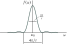
\includegraphics[scale=1]{figures/ch_17/fig_17_5.pdf}
		\caption[]{}
        % \caption[]{Graph depicting function $f(\omega)$ \eqref{eq:17_18}.}
		\label{fig:17_5}
	\end{center}
	\vspace{-0.9cm}
\end{figure}

Identifying $\tau$ with the coherence time, we arrive at the relation
\begin{equation}\label{eq:17_19}
    \ab{t}{coh} \sim \frac{1}{\Delta{\nu}}
\end{equation}

\noindent
(The sign $\sim$ stands for ``equal to in the order of magnitude'').

It can be seen from expression \eqref{eq:17_19} that the broader the interval of frequencies present in a given light wave, the smaller is the coherence time of this wave.

The frequency is related to the wavelength in a vacuum by the expression $\nu=c/\lambda_0$.
Differentiation of this expression yields $\Delta{\nu}=c\Delta{\lambda_0}/\lambda_0^2 \approx c \Delta{\lambda}/\lambda^2$ (we have omitted the minus sign obtained in differentiation and also assumed that $\lambda_0\approx\lambda$).
Substituting for $\Delta{\nu}$ in \eqn{17_19} its expression through $\lambda$ and $\Delta{\lambda}$, we obtain the following
expression for the coherence time:
\begin{equation}\label{eq:17_20}
    \ab{t}{coh} \sim \frac{\lambda^2}{c \Delta{\lambda}}.
\end{equation}

\noindent
Hence, we get the following value for the coherence length:
\begin{equation}\label{eq:17_21}
    \ab{l}{coh} = c \ab{t}{coh} \sim \frac{\lambda^2}{\Delta{\lambda}}.
\end{equation}

Examination of \eqn{17_5} shows that the path difference at which a maximum of the $m$-th order is obtained is determined by the relation
\begin{equation*}
    \Delta_m = \pm m \lambda_0 \approx \pm m \lambda.
\end{equation*}

\noindent
When this path difference reaches values of the order of the coherence length, the fringes become indistinguishable.
Consequently, the extreme interference order observed is determined by the condition
\begin{equation*}
    \ab{m}{extr} \lambda \sim \ab{l}{coh} \sim \frac{\lambda^2}{\Delta{\lambda}},
\end{equation*}

\noindent
whence
\begin{equation}\label{eq:17_22}
    \ab{m}{extr} \sim \frac{\lambda}{\Delta{\lambda}}.
\end{equation}

\noindent
It follows from \eqn{17_22} that the number of interference fringes observed according to the layout shown in \fig{17_2} grows when the wavelength interval in the light used diminishes.

\textbf{Spatial Coherence.}
According to the equation $k=\omega/v = n\omega/c$, scattering of the frequencies $\Delta{\omega}$ results in scattering of the values of $k$.
We have established that the temporal coherence is determined by the value of $\Delta{\omega}$.
Consequently, the temporal coherence is associated
with scattering of the values of the magnitude of the wave vector $\vec{k}$.
Spatial coherence is associated with scattering of the directions of the vector $\vec{k}$ that is characterized by the quantity $\Delta{\vecuni{k}}$.

The setting up at a certain point of space of oscillations produced by waves with different values of $\vecuni{k}$ is possible if these waves are emitted by different sections of an extended (not a point) light source.
Let us assume for simplicity's sake that the source has the form of a disk visible from a given point at the angle $\varphi$.
It can be seen from \fig{17_6} that the angle $\varphi$ characterizes the interval confining the
unit vectors $\vecuni{k}$.
We shall consider that this angle is small.

\begin{figure}[t]
	\begin{center}
		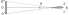
\includegraphics[scale=1]{figures/ch_17/fig_17_6.pdf}
		\caption[]{}
        % \caption[]{Waves emitted by different sections of an extended source with the form of a disk visible from a given point at the angle $\varphi$.}
		\label{fig:17_6}
	\end{center}
	\vspace{-0.9cm}
\end{figure}

Assume that the light from the source falls on two narrow slits behind which there is a screen (\fig{17_7}).
We shall consider that the interval of frequencies emitted by the source is very small.
This is needed for the degree of temporal coherence to be sufficient for obtaining a sharp interference pattern.
The wave arriving from the section of the surface designated in \fig{17_7} by $0$ produces a zero-order maximum M at the middle of the screen.
The zero-order maximum M$'$ produced by the wave arriving from section $0'$ will be displaced from the middle of the screen by the distance $x'$.
Owing to the smallness of the angle $\varphi$ and of the ratio $d/l$, we can consider that $x' = l\varphi/2$.
The zero-order maximum M$''$ produced by the wave arriving from section $0''$ is displaced in the opposite direction from the middle of the screen over the distance $x''$ equal to $x'$.
The zero-order maxima from the other sections of the source will be between the maxima M$'$ and M$''$.

The separate sections of the light source produce waves whose phases are in no way related to one another.
For this reason, the interference pattern appearing on the screen will be a superposition of the patterns produced by each section separately.
If the displacement $x'$ is much smaller than the width of an interference fringe $\Delta{x}=l\lambda/d$ [see \eqn{17_10}], then, the maxima from different sections of the source will practically be superposed on one another, and the pattern will be like the one produced by a point source.
When $x'\approx\Delta{x}$, the maxima from some sections will coincide with the minima from others, and no interference pattern will be observed.
Thus, an interference pattern will be distinguishable provided that $x'<\Delta{x}$, \ie,
\begin{equation}\label{eq:17_23}
    \frac{l \varphi}{2} < \frac{l \lambda}{d},
\end{equation}

\noindent
or
\begin{equation}\label{eq:17_24}
    \varphi < \frac{\lambda}{d}.
\end{equation}

\noindent
We have omitted the factor $2$ when passing over from expression \eqref{eq:17_23} to \eqref{eq:17_24}.

\begin{figure}[t]
	\begin{center}
		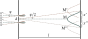
\includegraphics[scale=1]{figures/ch_17/fig_17_7.pdf}
		\caption[]{}
        % \caption[]{Interference pattern obtained from waves emitted through two slits. The source is that from \fig{17_6}.}
		\label{fig:17_7}
	\end{center}
	\vspace{-0.9cm}
\end{figure}

Formula \eqref{eq:17_24} determines the angular dimensions of a source at which interference is observed.
We can also use this formula to find the greatest distance between the slits at which interference from a source with the angular dimension $\varphi$ can still be observed.
Multiplying inequality \eqref{eq:17_24} by $d/\varphi$, we arrive at the condition
\begin{equation}\label{eq:17_25}
    d < \frac{\lambda}{\varphi}.
\end{equation}

A collection of waves with different values of $\vecuni{k}$ can be replaced with the resultant wave falling on a screen with slits.
The absence of an interference pattern signifies that the oscillations produced by this wave at the places where the first and second slits are situated are incoherent.
Consequently, the oscillations in the wave itself at points at a distance $d$ apart are incoherent too.
If the source were ideally monochromatic (this means that $\Delta{\nu}=0$ and $\ab{t}{coh}=\infty$), the surface passing through the slits would be a wave one, and the oscillations at all the points of this surface would occur in the same phase.
We have established that when $\Delta{v}\neq 0$ and the source has finite dimensions ($\varphi\neq 0$), the oscillations at points of a surface at a distance of $d>\lambda/\varphi$ are incoherent.

We shall call a surface, which would be a wave one if the source were monochromatic, a pseudowave surface\footnote{It must be borne in mind that this term is not used in scientific publications. The author has coined it for conditional use only to make the treatment
more illustrative.} for brevity.
We could satisfy condition \eqref{eq:17_24} by reducing the distance $d$ between the slits, \ie, by taking closer points of the pseudowave surface.
Consequently, oscillations produced by a wave at adequately close points of a pseudowave surface are coherent.
Such coherence is called \textbf{spatial}.
Thus, the phase of an oscillation changes chaotically when passing from one point of a pseudowave surface to another.
Let us introduce the distance $\ab{\rho}{coh}$, upon displacement by which along a pseudowave
surface a random change in the phase reaches a value of about $\pi$.
Oscillations at two points of a pseudowave surface spaced apart at a distance less than $\ab{\rho}{coh}$ will be approximately coherent.
The distance $\ab{\rho}{coh}$ is called the \textbf{spatial coherence length} or the \textbf{coherence radius}.
It can be seen from expression \eqref{eq:17_25} that
\begin{equation}\label{eq:17_26}
    \ab{\rho}{coh} \sim \frac{\lambda}{\varphi}.
\end{equation}

The angular dimension of the Sun is about $0.01$ radians, and the length of its light waves is about \SI{0.5}{\micro\metre}.
Hence, the coherence radius of the light waves arriving from the Sun has a value of the order of
\begin{equation}\label{eq:17_27}
    \ab{\rho}{coh} = \frac{0.5}{0.01} = \SI{50}{\micro\metre} = \SI{0.05}{\milli\metre}.
\end{equation}

The entire space occupied by a wave can be divided into parts in each of which the wave approximately retains coherence.
The volume of such a part of space, called the \textbf{coherence volume}, in its order of
magnitude equals the product of the temporal coherence length and the area of a circle of radius $\ab{\rho}{coh}$.

The spatial coherence of a light wave near the surface of the heated body emitting it is restricted by a value of $\ab{\rho}{coh}$ of only a few wavelengths.
With an increasing distance from the source, the degree of spatial coherence grows.
The radiation of a laser\footnote{Lasers will be treated in Vol. III of our course.} has an enormous temporal and spatial coherence.
At the outlet opening of a laser, spatial coherence is observed throughout the entire cross section of the light beam.

It would seem possible to observe interference by passing light propagating from an arbitrary source through two slits in an opaque screen.
With a small spatial coherence of the wave falling on the slits, however, the beams of light passing through them will be incoherent, and an interference pattern will be absent.
The English scientist Thomas Young (1773-1829) in 1802 obtained interference from two slits by increasing the spatial coherence of the light falling on the slits.
Young achieved such an increase by first passing the light through a small aperture in an opaque screen.
This light was used to illuminate the slits in a second opaque screen.
Thus, for the first time in history, Young observed the interference of light waves and determined the lengths of these waves.

\section{Ways of Observing the Interference of Light}\label{sec:17_3}

Let us consider two concrete interference layouts of which one uses reflection for splitting a light wave into two parts, and the other refraction of light.

\textbf{Fresnel's Double Mirror.}
Two plane contacting mirrors $0$M and $0$N are arranged so that their reflecting surfaces form an obtuse angle close to $\pi$ (\fig{17_8}).
Hence, the angle $\varphi$ in the figure is very small.
A straight light source S (for example, a narrow luminous slit) is placed parallel to the line of intersection of the mirrors $0$ (perpendicular
to the plane of the drawing) at a distance $r$ from it.
The mirrors reflect two cylindrical coherent waves onto screen Sc.
They propagate as if they were emitted by virtual sources S$_1$ and S$_2$.
Opaque screen Sc$_1$ prevents the direct propagation of the light from source S to screen Sc.

\begin{figure}[t]
	\begin{center}
		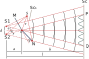
\includegraphics[scale=0.98]{figures/ch_17/fig_17_8.pdf}
		\caption[]{}
        % \caption[]{Fresnel's double mirror experiment. A light source S is placed parallel to the line of intersection of the mirrors $0$, reflecting two cylindrical coherent waves onto screen Sc. Opaque screen Sc$_1$ prevents the direct propagation of the light from source S to screen Sc.}
		\label{fig:17_8}
	\end{center}
	\vspace{-0.9cm}
\end{figure}

Ray $0$Q is the reflection of ray S$0$ from mirror $0$M, and ray $0$P is the reflection of ray S$0$ from mirror $0$N.
It is easy to see that the angle between rays $0$P and $0$Q is $2\varphi$.
Since S and S$_1$ are symmetrical relative to $0$M, the length of segment $0$S$_1$ equals $0$S, \ie, $r$.
Similar reasoning leads to the same result for segment $0$S$_2$.
Thus, the distance between sources S$_1$ and S$_2$ is
\begin{equation*}
    d = 2r \sin\varphi \approx 2 r \varphi.
\end{equation*}

\noindent
Inspection of \fig{17_8} shows that $a=r \cos\varphi \approx r$.
Hence,
\begin{equation*}
    l = r + b,
\end{equation*}

\noindent
where $b$ is the distance from the line of intersection of the mirrors $0$ to screen Sc.

Using the values of $d$ and $l$ we have found in \eqn{17_10}, we obtain the width of an interference fringe:
\begin{equation}\label{eq:17_28}
    \Delta{x} = \frac{r + b}{2 r \varphi} \lambda.
\end{equation}

\noindent
The region of wave overlapping PQ has a length of $2b\tan\varphi\approx 2b\varphi$.
Dividing this length by the width of a fringe $\Delta{x}$, we find the maximum number of interference fringes that can be observed with the
aid of Fresnel's double mirror at the given parameters of a layout:
\begin{equation}\label{eq:17_29}
    N = \frac{4 b r \varphi^2}{\lambda (r + b)}.
\end{equation}

\noindent
For all these fringes to be visible indeed, it is essential that $N/2$ be not greater than $\ab{m}{extr}$ determined by expression \eqref{eq:17_22}.

\textbf{Fresnel's Biprism}.
Two prisms with a small refracting angle $\theta$ made from a single piece of glass have one common face (\fig{17_9}).
A straight light source S is arranged parallel to this face at a distance a from it.

\begin{figure}[t]
	\begin{center}
		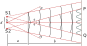
\includegraphics[scale=0.98]{figures/ch_17/fig_17_9.pdf}
		\caption[]{}
        % \caption[]{Fresnel's biprism experiment. Two prisms with a small refracting angle $\theta$ made from a single piece of glass have one common face. A straight light source S is arranged parallel to this face at a distance a from it.}
		\label{fig:17_9}
	\end{center}
	\vspace{-0.9cm}
\end{figure}

It can be shown that when the refracting angle a of the prism is very small and the angles of incidence of the rays on the face of the prism are not very great, all the rays are deflected by the prism through a practically identical angle equal to
\begin{equation*}
    \varphi = (n - 1) \theta
\end{equation*}

\noindent
($n$ is the refractive index of the prism).
The angle of incidence of the rays on the biprism is not great.
Therefore, all the rays are deflected by each half of the biprism through the same angle.
As a result, two coherent cylindrical waves are formed emerging from virtual sources S$_1$ and S$_2$ in the same plane as S.
The distance between the sources is
\begin{equation*}
    d = 2a \sin\varphi \approx 2a\varphi = 2a (n - 1) \theta.
\end{equation*}

\noindent
The distance from the sources to the screen is
\begin{equation*}
    l = a + b.
\end{equation*}

We find the width of an interference fringe by \eqn{17_10}:
\begin{equation}\label{eq:17_30}
    \Delta{x} = \frac{(a + b)}{2 a (n - 1) \theta} \lambda.
\end{equation}

\noindent
The region of overlapping of the waves PQ has the length
\begin{equation*}
    2b \tan\varphi \approx 2b\varphi = 2b (n - 1) \theta.
\end{equation*}

\noindent
The maximum number of fringes observed is
\begin{equation}\label{eq:17_31}
    N = \frac{4ab (n-1)^2 \theta^2}{\lambda (a+b)}.
\end{equation}

\section{Interference of Light Reflected from Thin Plates}\label{sec:17_4}

When a light wave falls on a thin transparent plate (or film), reflection occurs from both surfaces of the plate.
The result is the production of two light waves that in known conditions can interfere.

Assume that a plane light wave which can be considered as a parallel beam of rays falls on a transparent plane-parallel plate (\fig{17_10}).
The plate reflects upward two parallel beams of light.
One of them was formed as a result of reflection from the top surface of the plate and the second as a result of reflection from its bottom surface (in \fig{17_10} each of these beams is  represented by only one ray).
The second beam is refracted when it enters the plate and leaves it.
In addition to these two beams, the plate throws upward beams produced as a result of three-, five-fold, etc. reflection from the plate surfaces.
Owing to their small intensity, however, we shall take no account of these beams\footnote{At $n=1.5$, about $5\%$ of the incident luminous flux is reflected from the surface of the plate (see the last paragraph of \sect{16_3}). After two reflections, the intensity will be $0.05\times 0.05$ or $0.25\%$ of the intensity of the initial beam. After three reflections, the relevant figure is $0.05\times 0.05\times 0.05$, or $0.0125\%$, which is $1/400$ of the intensity of the singly reflected beam.}.
We shall also display no interest in the beams passing through the plate.

\begin{figure}[t]
	\begin{center}
		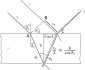
\includegraphics[scale=0.95]{figures/ch_17/fig_17_10.pdf}
		\caption[]{}
        % \caption[]{Interference of light in a parallel-plate.}
		\label{fig:17_10}
	\end{center}
	\vspace{-0.8cm}
\end{figure}

The path difference acquired by rays $1$ and $2$ before they meet at point C is
\begin{equation}\label{eq:17_32}
    \Delta = ns_2 - s_1,
\end{equation}

\noindent
where $s_1$ is the length of segment BC, $s_2$ is the total length of segments AO and OC and $n$ the refractive index of the plate.

We assume that the refractive index of the medium surrounding the plate is unity.
A glance at \fig{17_10} shows that $s_1 = 2b \tan\theta_2 \times \sin\theta_1$, and $s_2=2b/\cos\theta_2$ (here, $b$ is the thickness of the plate).

Using these values in \eqn{17_32}, we get
\begin{equation*}
    \Delta = \frac{2bn}{\cos\theta_2} - 2b\tan\theta_2\sin\theta_1 = 2b \frac{n^2 - n \sin\theta_2 \sin\theta_1}{n \cos\theta_2}.
\end{equation*}

\noindent
Substituting $\sin\theta_1$ for $n\sin\theta_1$ and taking into account that
\begin{equation*}
    n \cos\theta_2 = \sqrt{n^2 - n^2 \sin^2\theta_2} = \sqrt{n^2 - \sin^2\theta_1},
\end{equation*}

\noindent
it is easy to give the equation for $\Delta$ the form
\begin{equation}\label{eq:17_33}
    \Delta = 2b \sqrt{n^2 - \sin^2\theta_1}.
\end{equation}

When calculating the phase difference $\delta$ between the oscillations in rays $1$ and $2$, it is necessary, in addition to the optical path difference $\Delta$, to take into account the possibility of a change in the phase of the wave upon reflection (see \sect{16_3}).
At point A (see \fig{17_10}), reflection occurs from the interface between the optically less dense medium and the optically denser one.
Consequently, the wave phase experiences a change by $\pi$.
At point $0$, reflection occurs from the interface between the optically denser medium and the optically less dense one, so that there is no jump in the phase.
Hence, an additional phase difference equal to $\pi$ is produced between rays $1$ and $2$.
It can be taken into account by adding to $\Delta$ (or subtracting from it) half a wavelength in a vacuum. The result is
\begin{equation}\label{eq:17_34}
    \Delta = 2 b \sqrt{n^2 - \sin^2\theta_1} - \frac{\lambda_0}{2}.
\end{equation}

Thus, when a plane wave falls on the plate, two reflected waves are formed, and their path difference is determined by \eqn{17_34}.
Let us determine the conditions in which these waves will be coherent and can interfere.
We shall consider two cases.

\textbf{1. A Plane-Parallel Plate.}
Both plane reflected waves propagate in one direction making an angle equal to the angle of incidence $\theta_1$ with a normal to the plate.
These waves can interfere if conditions of both temporal and spatial coherence are observed.

For temporal coherence to take place, the path difference given by \eqn{17_34} must not exceed the coherence length equal to $\lambda^2/\Delta{\lambda}\approx\lambda_0^2/\Delta{\lambda_0}$ [see expression \eqref{eq:17_21}].
Consequently, the condition
\begin{equation*}
    2b \sqrt{n^2 - \sin^2\theta_1} - \frac{\lambda_0}{2} < \frac{\lambda_0^2}{\Delta{\lambda_0}},
\end{equation*}

\noindent
or
\begin{equation*}
    b < \frac{\lambda_0 (\lambda_0/\Delta{\lambda_0} + 1/2)}{2 \sqrt{n^2 - \sin^2\theta_1}},
\end{equation*}

\noindent
must be observed.
In the obtained relation, we may disregard $1/2$
in comparison with $\lambda_0/\Delta{\lambda_0}$.
The expression $\sqrt{n^2-\sin^2\theta_1}$ has a magnitude of the order of unity\footnote{For $n=1.5$, the magnitude of this expression varies within the limits from $1.12$ (at $\theta_1=\pi/2$) to $1.5$ (at $\theta_1=0$).}.
We can therefore write
\begin{equation}\label{eq:17_35}
    b < \frac{\lambda_0^2}{2 \Delta{\lambda_0}}
\end{equation}

\noindent
(the double plate thickness must be less than the coherence length).

Thus, the reflected waves will be coherent only if the plate thickness $b$ does not exceed the value determined by expression \eqref{eq:17_35}.
Assuming that $\lambda_0=\SI{5000}{\angstrom}$ and $\Delta{\lambda_0}=\SI{20}{\angstrom}$, we get the extreme value of the thickness equal to
\begin{equation}\label{eq:17_36}
    \frac{5000^2}{2 \times 20} \approx \SI{6e5}{\angstrom} = \SI{0.06}{\milli\metre}.
\end{equation}

Now, let us consider the conditions for observance of spatial coherence.
Let us place screen Sc in the path of the reflected beams (\fig{17_11}).
Rays $1'$ and $2'$ arriving at point P$'$ will be at a distance $\rho'$ apart in the incident beam.
If this distance does not exceed the coherence radius $\ab{\rho}{coh}$ of the incident wave, rays $1'$ and $2'$ will be coherent and will produce at point P$'$ an illumination determined by the value of the path difference $\Delta$ corresponding to the angle of incidence $\theta_1$.
The other pairs of rays travelling at the same angle $\theta_1'$ will produce the same illumination at the other points of the screen.
The screen will thus be uniformly illuminated (in the particular case when $\Delta=(n+1/2)\lambda_0$, the screen will be dark).
When the inclination of the beam is changed (\ie, when the angle $\theta_1$ is changed), the illumination of the screen will change too.

\begin{figure}[t]
	\begin{center}
		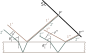
\includegraphics[scale=1]{figures/ch_17/fig_17_11.pdf}
		\caption[]{}
        % \caption[]{Spatial coherence in a plane-parallel plate. Rays $1'$ and $2'$ arriving at point P$'$ will be at a distance $\rho'$ apart in the incident beam. If $\rho'<\ab{\rho}{coh}$ of the incident wave, rays $1'$ and $2'$ will be coherent and will produce at point P$'$ an illumination determined by the value of the path difference $\Delta$ corresponding to the angle of incidence $\theta_1$.}
		\label{fig:17_11}
	\end{center}
	\vspace{-0.8cm}
\end{figure}

A glance at \fig{17_10} shows that the distance between the incident rays $1$ and $2$ is
\begin{equation}\label{eq:17_37}
    \rho = 2b\tan\theta_2\sin\theta_1 = \frac{b \sin(2\theta_1)}{\sqrt{n^2 - \sin^2\theta_1}}.
\end{equation}

\noindent
If we assume that $n=1.5$, then, for $\theta_1=\SI{45}{\degree}$ we get $\rho=0.8b$, and for $\theta_1=\SI{10}{\degree}$ we get $\rho=0.1b$.
For normal incidence ($\theta_1=0$), we have $\rho=0$ at any $n$.

The coherence radius of sunlight has a value of the order of \SI{0.05}{\milli\metre} [see \eqn{17_27}].
At an angle of incidence of \SI{45}{\degree}, we may assume that $\rho\approx b$.
Hence, for interference to occur in these conditions, the relation
\begin{equation}\label{eq:17_38}
    b < \SI{0.05}{\milli\metre}
\end{equation}

\noindent
must be observed [compare with \eqn{17_36}].
For an angle of incidence of about \SI{10}{\degree}, spatial coherence will be retained at a plate thickness not exceeding \SI{0.5}{\milli\metre}.
We thus arrive at the conclusion that owing to the restrictions imposed by temporal and spatial coherence, interference is observed when a plate is illuminated by sunlight only if the thickness of the plate does not exceed a few hundredths of a millimetre.
Upon illumination with light having a greater degree of coherence, interference is also observed in reflection from thicker plates or films.

Interference from a plane-parallel plate is observed in practice by placing in the path of the reflected beams a lens that gathers the rays at one of the points of the screen in the focal plane of the lens (\fig{17_12}).
The illumination at this point depends on the value of quantity \eqref{eq:17_34}.
When $\Delta=m\lambda_0$, we get maxima, and when $\Delta=(m+1/2)\lambda_0$---minima of the intensity ($m$ is an integer).
The condition for the maximum intensity has the form
\begin{equation}\label{eq:17_39}
    2b \sqrt{n^2 - \sin^2\theta_1} = \parenthesis{m + \frac{1}{2}} \lambda_0.
\end{equation}

\begin{figure}[t]
	\begin{center}
		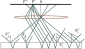
\includegraphics[scale=1]{figures/ch_17/fig_17_12.pdf}
		\caption[]{}
        % \caption[]{Interference from a plane-parallel plate observed by placing in the path of the reflected beams a lens that gathers the rays at one of the points of the screen in the focal plane of the lens.}
		\label{fig:17_12}
	\end{center}
	\vspace{-0.8cm}
\end{figure}

Assume that a thin plane-parallel plate is illuminated by diffuse monochromatic light (see \fig{17_12}).
Let us arrange a lens parallel to the plate and put a screen in the focal plane of the lens.
Diffuse light contains rays of the most diverse directions.
The rays parallel to the plane of the drawing and falling on the plate at the angle $\theta_1'$ after reflection from both surfaces of the plate will be gathered by the lens at point P$'$ and will set up at this point an illumination determined by the value of the optical path difference.
Rays propagating in other planes but falling on the plate at the same angle $\theta_1'$
will be gathered by the lens at other points at the same distance as point P$'$ from centre $0$ of the screen.
The illumination at all these points will be the same.
Thus, the rays falling on the plate at the same angle $\theta_1'$ will produce on the screen a collection of identically illuminated points arranged along a circle with its centre at $0$.
Similarly, the rays falling at a different angle $\theta_1''$ will produce on the screen a collection of identically (but different in value because $\Delta$ is different) illuminated points arranged along a circle of another radius.
The result will be the appearance on the screen of a system of alternating bright and dark circular fringes with a common centre at point $0$.
Each fringe is formed by the rays falling on the plate at the same angle $\theta_1$.
This is why interference fringes produced in such conditions are known as fringes of equal inclination.
When the lens is arranged differently relative to the plate (the screen must coincide with the focal plane of the lens in all cases), the fringes of equal inclination will have another shape.

Every point of an interference pattern is due to rays which formed a parallel beam before passing through the lens.
Hence, in observing fringes of equal inclination, the screen must be placed in the focal plane of the lens, \ie, in the same way in which it is arranged to produce an image of infinitely remote objects on it.
Accordingly, fringes of equal inclination are said to be localized at infinity.
The part of the lens can be played by the crystalline lens, and that of the screen by the retina of the eye.
In this case for observing fringes of equal inclination, the eye must be accommodated as when looking at very remote objects.

According to \eqn{17_39}, the position of the maxima depends on the wavelength $\lambda_0$.
Therefore, in white light, we get a collection of
fringes displaced relative to one another and formed by rays of different colours; the interference pattern acquires the colouring of a rainbow.
The possibility of observing an interference pattern in white light is determined by the ability of the eye to distinguish light tints of close wavelengths.
The average human eye perceives rays differing in wavelength by less than \SI{20}{\angstrom} as having the same colour.
Therefore, to assess the conditions in which interference from plates can be observed in white light, we must assume that $\Delta{\lambda_0}$ equals \SI{20}{\angstrom}.
We took exactly this value in assessing the thickness of a plate [see \eqn{17_36}].

\textbf{2. Plate of Varying Thickness.}
Let us take a plate in the form of a wedge with an apex angle of $\varphi$ (\fig{17_13}).
Assume that a parallel beam of rays falls on it.
Now the rays reflected from different surfaces of the plate will not be parallel.
Two rays that practically merge before falling on the plate (in \fig{17_13} they are depicted in the form of a single straight line designated by the figure $1'$) intersect after reflection at point $Q'$.
The two rays $1''$ practically merging intersect
at point Q$''$ after reflection.
It can be shown that points Q$'$, Q$''$ and other points similar to them lie in one plane passing through apex $0$ of the wedge.
Ray $1'$ reflected from the bottom surface of the wedge and ray $2'$ reflected from its top surface will intersect at point R$'$ that is closer to the wedge than Q$'$.
Similar rays $1'$ and $3'$ will intersect at point P$'$ that is farther from the wedge surface than Q$'$.

\begin{figure}[t]
	\begin{center}
		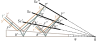
\includegraphics[scale=1]{figures/ch_17/fig_17_13.pdf}
		\caption[]{}
        % \caption[]{Interference of rays in a plate of varying thickness (wedge).}
		\label{fig:17_13}
	\end{center}
	\vspace{-0.8cm}
\end{figure}

The directions of propagation of the waves reflected from the top and bottom surfaces of the wedge do not coincide.
Temporal coherence will be observed only for the parts of the waves reflected from places of the wedge for which the thickness satisfies condition \eqref{eq:17_35}.
Assume that this condition is observed for the entire wedge.
In addition, assume that the coherence radius is much greater than the wedge length.
Hence, the reflected waves will be coherent in the entire space over the wedge, and no matter at what distance from the wedge the screen is, an interference pattern will be observed on it in the form of fringes parallel to the wedge apex $0$ (see the last three paragraphs of \sect{17_1}).
This, particularly, is how matters are when a wedge is illuminated by light emitted by a laser.

With restricted spatial coherence, the region of localization of the interference pattern (\ie, the region of space in which an interference pattern can be seen on a screen placed in it) will be restricted too.
If we arrange a screen so that it pass.3s through points Q$'$, Q$''$, $\ldots$ (see screen Sc in \fig{17_13}), an interference pattern will appear on it even if the spatial coherence of the falling wave is extremely small (rays that coincided before falling on the wedge will intersect at points on the screen).
At a small wedge angle $\varphi$, the path difference of the rays can be calculated with sufficient accuracy by \eqn{17_34} taking as $b$ the thickness of the plate at the place where the rays fall on it.
Since the path difference for the rays reflected from different sections of the wedge is now different, the illumination of the screen will be non-uniform---bright and dark fringes will appear on it (see the dash curve showing the illumination of screen Sc in \fig{17_13}).
Each of these fringes is produced as a result of reflection from sections of the wedge having the same thickness.
This is why they are known as \textbf{fringes of equal thickness}.

Upon displacement of the screen from position Sc in a direction away from the wedge or toward it, the degree of spatial coherence of the incident wave begins to tell.
If in the position of the screen denoted in \fig{17_13} by Sc$'$, the distance $\rho'$ between the incident rays $1'$ and $2'$ becomes of the order of the coherence radius, no interference pattern will be observed on screen Sc$'$.
Similarly, the pattern vanishes when the screen is at position Sc$''$.

Thus, the interference pattern produced when a plane wave is reflected from a wedge is localized in a certain region near the surface of the wedge.
This region becomes narrower when the degree of spatial coherence of the incident wave diminishes.
Inspection of \fig{17_13} shows that the conditions for both temporal and spatial coherence
become more favourable nearer to the apex of the wedge.
Therefore, the distinctness of the interference pattern diminishes when moving from the apex of the wedge to its base.
A pattern may be observed only for the thinner part of the wedge.
For its remaining part, the screen will be uniformly illuminated.

\begin{figure}[t]
	\begin{center}
		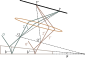
\includegraphics[scale=0.9]{figures/ch_17/fig_17_14.pdf}
		\caption[]{}
        % \caption[]{Fringes of equal thickness are observed by placing a lens near a wedge, and a screen behind the lens.}
		\label{fig:17_14}
	\end{center}
	\vspace{-0.8cm}
\end{figure}

Practically, fringes of equal thickness are observed by placing a lens near a wedge, and a screen behind the lens (\fig{17_14}).
The part of the lens can be played by the crystalline lens, and of the screen by the retina of the eye.
If the screen behind the lens is in a plane conjugated with the plane designated by Sc in \fig{17_13} (the eye is accordingly accommodated to this plane), the pattern will be most distinct.
When the screen onto which the image is projected is moved (or when the lens is moved), the pattern will become less distinct and will vanish completely if the plane conjugated with the screen passes beyond the limits of the region of localization of the interference pattern observed without a lens.

When observed in white light, the fringes will be coloured, so that the surface of a plate or film will have rainbow colouring.
For example, thin films of oil on the surface of water and soap films have such colouring.
The temper colours appearing on the surface of steel articles when they are hardened are also due to interference from a film of transparent oxides.

Let us compare the two cases of interference upon reflection from thin films which we have considered.
Fringes of equal inclination are obtained when a
plate of constant thickness ($b=\text{constant}$) is illuminated by diffuse light containing
rays of various directions ($\theta_1$ is varied within more or less broad limits).
Fringes of equal inclination are localized at infinity.
Fringes of equal thickness are observed when a plate of varying thickness ($b$ varies) is illuminated by a parallel beam of light ($\theta_1=\text{constant}$).
Fringes of equal thickness are localized near the plate.
In real conditions, for example, when observing rainbow colours on a soap or oil film, both the angle of incidence of the rays and the thickness of the film are varied.
In this case, fringes of a mixed type are observed.

We must note that interference from thin films can be observed not only in reflected, but also in transmitted light.

\textbf{Newton's Rings.}
A classical example of fringes of equal thickness
are \textbf{Newton's rings}.
They are observed when light is reflected from a thick plane-parallel glass plate in contact with a plano-convex lens having a large radius of curvature (\fig{17_15}).
The part of a thin film from whose surfaces coherent waves are reflected is played by the air gap between the plate and the lens (owing to the great thickness of the plate and the lens, no interference fringes appear as a result of reflections from other surfaces).
With normal incidence of the light, fringes of equal thickness have the form of concentric rings, and with inclined incidence, of ellipses.
Let us find the radii of Newton's rings produced when light falls along a normal to the plate.
In this case, $\sin\theta_1=0$, and the optical path difference equals the double thickness of the gap [see \eqn{17_33}, it is assumed that $n=1$ in the gap].
It follows from \fig{17_15} that
\begin{equation}\label{eq:17_40}
    R^2 = (R - b)^2 + r^2 \approx R^2 - 2Rb + r^2,
\end{equation}

\noindent
where $R$ is the radius of curvature of the lens, $r$ is the radius of a circle with the identical gap $b$ corresponding to all of its points.

\begin{figure}[t]
	\begin{center}
		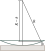
\includegraphics[scale=1]{figures/ch_17/fig_17_15.pdf}
		\caption[]{}
        % \caption[]{Newton's rings are observed when light is reflected from a thick plane-parallel glass plate in contact with a plano-convex lens having a large radius of curvature.}
		\label{fig:17_15}
	\end{center}
	\vspace{-0.8cm}
\end{figure}

Owing to the smallness of $b$, in expression \eqref{eq:17_40} we have disregarded the quantity $b^2$ in comparison with $2Rb$.
In accordance with expression \eqref{eq:17_40}, $b=r^2/(2R)$.
To take account of the change in the phase by $\pi$ occurring upon reflection from the plate, we must add $\lambda_0/2$ to $2b=r^2/R$.
The result is
\begin{equation}\label{eq:17_41}
    \Delta = \frac{r^2}{R} + \frac{\lambda_0}{2}.
\end{equation}

At points for which $\Delta=m'\lambda_0 = 2m'(\lambda_0/2)$, maxima appear, and at points for which $\Delta=(m'+1/2) \lambda_0 = (2m'+1)(\lambda_0/2)$, minima of the intensity appear.
Both conditions can be combined into the single one
\begin{equation*}
    \Delta = m \frac{\lambda_0}{2}
\end{equation*}

\noindent
maxima corresponding to even values of $m$, and minima of the intensity, to odd values.
Introducing into this expression \eqn{17_41} for $\Delta$ and solving the resulting equation relative to $r$, we find the radii of bright and dark Newton's rings:
\begin{equation}\label{eq:17_42}
    r = \parenthesis{\frac{R \lambda_0 (m-1)}{2}}^{1/2}\quad (m = 1, 2, 3, \ldots).
\end{equation}

\noindent
Radii of bright rings correspond to even $m$'s, and radii of dark rings to odd ones.
The value $r=0$ corresponds to $m=1$, \ie, to the point at the place of contact of the plate and the lens.
A minimum of intensity is observed at this point.
It is due to the change in the phase by $\pi$ when a light wave is reflected from the plate.

\textbf{Coating of Lenses.}
The coating of lenses is based on the interference of light when reflected from thin films.
The transmission of light through each refracting surface of a lens is attended by the reflection of about four per cent of the incident light.
In multicomponent lenses, such reflections occur many times, and the total loss of the light flux reaches an appreciable value.
In addition, the reflections from the lens surfaces result in the appearance of highlights.
The reflection of light is eliminated by applying a thin film of a substance having a refractive index other than that of the lens to each free surface of the latter.
The components obtained in this way are called \textbf{coated lenses}.
The thickness of the coating is chosen so that the waves reflected from both its surfaces interfere destructively.
An especially good result is obtained if the refractive index of the film equals the square root of the refractive index of the lens.
When this condition is satisfied, the intensity of both waves reflected from the film surfaces is the same.

\section{The Michelson Interferometer}\label{sec:17_5}

Many varieties of interference instruments called \textbf{interferometers} are in use.
Figure \ref{fig:17_16} is a schematic view of a \textbf{Michelson interferometer}\footnote{Named after its inventor, the American physicist Albert Michelson (1852-1931).}.
A light beam from source S falls on semitransparent plate P$_1$ coated with a thin layer of silver (this layer is depicted by dots in the figure).
Half of the incident light flux is reflected by plate P$_1$ in the direction of ray $1$ and half passes through the plate and propagates in the direction of ray $2$. Beam $1$ is reflected from mirror M$_1$ and returns to P$_1$, where it is split into two beams of equal intensity.
One of them passes through the plate and forms beam $1'$, and the second one is reflected in the direction of S.
The latter beam will no longer interest us.
Beam $2$ after being reflected by mirror M$_2$ also returns to plate P$_1$ where it is divided into two parts: beam $2'$ reflected from the semitransparent layer, and the beam transmitted through the layer, which will also no longer interest us.
Light beams $1'$ and $2'$ have the same intensity.

\begin{figure}[t]
	\begin{center}
		\includegraphics[scale=1]{figures/ch_17/fig_17_16.pdf}
		\caption[]{}
        % \caption[]{(a) Scheme of the Michelson interferometer. Light travels from the source S and pass through the beam splitters P$_1$ and P$_2$, and is reflected by the mirrors M$_1$ and M$_2$. After multiple reflections, the rays are collected by the detector T. (b) The movable mirrors allow to change the thickness of the ``plate''; in particular, we can make planes M$_1$ and M$_2$ intersect.}
		\label{fig:17_16}
	\end{center}
	\vspace{-0.8cm}
\end{figure}

If conditions of temporal and spatial coherence are observed, beams $1'$ and $2'$ will interfere.
The result of this interference depends on the optical path difference from plate P$_1$ to mirrors M$_1$ and M$_2$, and back.
Ray $2$ passes through the plate three times, and ray $1$ only once.
To compensate the resulting change in the optical path difference (owing to dispersion) for waves of different lengths, plate P$_1$ is placed in the path of ray $1$.
Plates P$_1$ and P$_2$ are identical, except for the silver coating on the former.
This arrangement makes the paths of rays $1$ and $2$ in glass equal.
The interference pattern is observed with the aid of telescope T.

Let us mentally replace mirror M$_2$ with its virtual image M$_2'$ in semitransparent plate P$_1$.
Beams $1'$ and $2'$ can thus be considered as due to reflection from a transparent plate contained between planes M$_1$ and M$_2$.
We can use adjusting screws W$_1$ to change the angle between these planes; in particular, they can be arranged strictly parallel to each other.
By rotating micrometric screw W$_2$, we can smoothly move mirror M$_1$ without changing its inclination.
We can thus change the thickness of the ``plate''; in particular, we can make planes M$_1$ and M$_2$ intersect (\fig{17_16}b).

The nature of the interference pattern depends on the adjustment of the mirrors and on the divergence of the beam of light falling on the instrument.
If the beam is parallel, and planes M$_1$ and M$_2$ make an angle other than zero, then straight fringes of equal thickness parallel to the lines of intersection of planes M$_1$ and M$_2$ will be observed in the field of vision of the telescope.
In white light, all the fringes except the one coinciding with the line of intersection of the zero-order fringe will be coloured.
The zero-order fringe will be black because beam $1$ is reflected from plate P$_1$ from the outside, and beam $2$ from the inside.
As a result, a phase difference equal to $\pi$ is produced between them.
In white light, fringes are observed only with a small thickness of ``plate'' M$_1$M$_2'$ [see \eqn{17_36}].
In monochromatic light corresponding to the red line of cadmium, Michelson observed a distinct interference pattern at a path difference of the order of $500000$ wavelengths (the distance between M$_1$ and M$_2'$ in this case is about \SI{150}{\milli\metre}).

With a slightly diverging beam of light and a strictly parallel arrangement of planes M$_1$ and M$_2'$, fringes of equal inclination are obtained that have the form of concentric rings.
When micrometric screw W$_2$ is rotated, the diameter of the rings grows or diminishes.
Either new rings appear at the centre of the pattern, or the diminishing rings shrink to a point and then vanish.
Displacement of the pattern by one fringe corresponds to movement of mirror M$_2$ through half a wavelength.

Michelson used the instrument described above to carry out several experiments that entered the annals of physics.
The most famous of them, performed together with the American chemist Edward Morley (1838-1923) in 1887, had the aim of detecting motion of the Earth relative to the hypothetic ether (we shall treat this experiment in \sect{21_3}).
In 1890-1895, Michelson used the interferometer he had invented to make the first comparison of the wavelength of the red line of cadmium with the length of the standard metre.

In 1920, Michelson constructed a \textbf{stellar interferometer} which he used to measure the angular dimensions of stars.
This instrument was mounted on a telescope.
A screen with two slits was installed in front of the objective of the telescope (\fig{17_17}).
The light from a star was reflected from a symmetrical system of mirrors M$_1$, M$_2$, M$_3$ and M$_4$, installed on a rigid frame fastened on a carriage.
The inner mirrors M$_3$ and M$_4$, were fixed, and the outer ones M$_1$ and M$_2$, could move symmetrically away from or toward mirrors M$_3$ and M$_4$.
The path of the rays is clear from the figure.
Interference fringes were produced in the focal plane of the telescope objective.
Their visibility\footnote{The visibility of a fringe is defined as the quantity $V = (\ab{I}{max}-\ab{I}{min})/(\ab{I}{max}+\ab{I}{min})$, where $\ab{I}{max}$ and $\ab{I}{min}$ are the maximum and minimum intensities of the light in the vicinity of the given fringe, respectively.} depended on the distance between the outer mirrors.
By moving these mirrors, Michelson determined the distance $l$ between them at which the visibility of the fringes vanishes.
This distance must be of the order of the coherence radius of a light wave arriving from a star.
According to expression \eqref{eq:17_26}, the coherence radius is $l=\lambda/\varphi$.
The condition $l=\lambda/\varphi$ gives the angular diameter of a star
\begin{equation*}
    \varphi = \frac{\lambda}{l}.
\end{equation*}

\begin{figure}[t]
	\begin{center}
		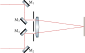
\includegraphics[scale=0.9]{figures/ch_17/fig_17_17.pdf}
		\caption[]{}
        % \caption[]{Scheme of the stellar interferometer used by Michelson to measure the angular dimensions of stars.}
		\label{fig:17_17}
	\end{center}
	\vspace{-0.8cm}
\end{figure}

\noindent
Accurate calculations give the formula
\begin{equation*}
    \varphi = A \frac{\lambda}{l},
\end{equation*}

\noindent
where $A=1.22$ for a source in the form of a uniformly illuminated disk.
If the disk is darker at its edges than at the centre, the coefficient exceeds $1.22$, its value depending on the rate of diminishing of the illumination in the direction from the centre toward the edge.
In addition, accurate calculations show that after vanishing at a certain value of $l$, the visibility upon a further increase in $l$ again
becomes other than zero; however, the values it reaches are not great.

The maximum distance between the outer mirrors in the stellar interferometer constructed by Michelson was \SI{6.1}{\metre} (the diameter
of the telescope was \SI{2.5}{\metre}).
A minimum measurable angular diameter of about \ang{;0.02;} corresponded to this distance.
The first star whose angular diameter was measured was Betelgeuse (alpha Orion).
The value of $\varphi$ obtained for it was \ang{;0.047;}.

\section{Multibeam Interference}\label{sec:17_6}

Up to now, we have dealt with two-beam interference.
Now let us investigate the interference of many light rays.

Assume that $N$ rays of the same intensity arrive at a given point of a screen, the phase of each following ray being shifted relative
to that of the preceding one by the same value $\delta$.
Let us represent the oscillations set up by the rays in the form of exponents:
\begin{equation*}
    E_1 = a e^{i\omega t},\, E_2 = a e^{i(\omega t+\delta)}, \ldots, E_m = a e^{i[\omega t+(m-1)\delta]},\ldots, E_N = a e^{i[\omega t+(N-1)\delta]},
\end{equation*}

\noindent
where $a$ is the amplitude of an oscillation.
The resultant oscillation is determined by the formula
\begin{equation*}
    E = \sum_{m=1}^N E_m = a e^{i\omega t} \sum_{m=1}^N e^{i (m-1) \delta}.
\end{equation*}

\noindent
The expression obtained is the sum of $N$ terms of a geometrical progression with its first term equal to unity and its common ratio equal to $e^{i\delta}$.
Hence,
\begin{equation*}
    E = a e^{i\omega t} \parenthesis{\frac{1 - e^{iN\delta}}{1 - e^{i\delta}}} = \hat{A}\, e^{i\omega t},
\end{equation*}

\noindent
where
\begin{equation}\label{eq:17_43}
    \hat{A} = a \parenthesis{\frac{1 - e^{iN\delta}}{1 - e^{i\delta}}},
\end{equation}

\noindent
is the complex amplitude that can be represented in the form
\begin{equation}\label{eq:17_44}
    \hat{A} = A e^{i\alpha},
\end{equation}

\noindent
($A$ is the usual amplitude of the resultant oscillation, and $\alpha$ is its initial phase).

The product of quantity \eqref{eq:17_44} and its complex conjugate gives the square of the amplitude of the resultant oscillation:
\begin{equation}\label{eq:17_45}
    \hat{A}\hat{A}^* = A e^{i\alpha} A e^{-i\alpha} = A^2.
\end{equation}

\noindent
Substituting for $A$ in \eqn{17_45} its value from \eqn{17_43}, we get the following expression for the square of the amplitude:
\begin{align}
    A^2 &= \hat{A}\hat{A}^* = a^2 \frac{ \parenthesis{1 - e^{iN\delta}} \parenthesis{1 - e^{-iN\delta}} }{ \parenthesis{1 - e^{i\delta}} \parenthesis{1 - e^{-i\delta}}} = a^2 \frac{ \parenthesis{2 - e^{iN\delta} - e^{-iN\delta}} }{ \parenthesis{2 - e^{i\delta} - e^{-i\delta}} } \nonumber\\
    & = a^2 \bracket{ \frac{1 - \cos(N\delta)}{1 - \cos\delta} } = a^2 \frac{\sin^2(N\delta/2)}{\sin^2(\delta/2)}. \label{eq:17_46}
\end{align}

The intensity is proportional to the square of the amplitude.
Hence, the intensity produced upon the interference of the $N$ rays being considered is determined by the expression
\begin{equation}\label{eq:17_47}
    I(\delta) = K a^2 \frac{\sin^2(N\delta/2)}{\sin^2(\delta/2)} = I_0 \frac{\sin^2(N\delta/2)}{\sin^2(\delta/2)}
\end{equation}

\noindent
($K$ is a constant of proportionality, $I_0=Ka^2$ is the intensity produced by each of the rays separately).

At the values
\begin{equation}\label{eq:17_48}
    \delta = 2 \pi m \quad (m = 0, \pm 1, \pm 2, \ldots),
\end{equation}

\noindent
\eqn{17_47} becomes indeterminate.
For this reason, we apply L'Hospital's rule:
\begin{equation*}
    \lim_{\delta\to 2\pi m} \frac{\sin^2(N\delta/2)}{\sin^2(\delta/2)} = \lim_{\delta\to 2\pi m} \frac{ 2 \sin(N\delta/2) \cos(N\delta/2) (N/2)}{ 2 \sin(\delta/2) \cos(\delta/2) (1/2) } = \lim_{\delta\to 2\pi m} N \frac{ \sin(N\delta) }{\sin\delta}.
\end{equation*}

\noindent
The expression obtained is also indeterminate.
For this reason, we apply L'Hospital's rule again:
\begin{equation*}
    \lim_{\delta\to 2\pi m} \frac{\sin^2(N\delta/2)}{\sin^2(\delta/2)} = \lim_{\delta\to 2\pi m} N \frac{ \sin(N\delta) }{\sin\delta} = \lim_{\delta\to 2\pi m} N \frac{ \cos(N\delta) }{\cos\delta} = N^2.
\end{equation*}

Thus, when $\delta=2\pi m$ (or when the path differences $\Delta=m\lambda_0$), the resultant intensity is
\begin{equation}\label{eq:17_49}
    I = I_0 N^2.
\end{equation}

\noindent
This result could have been predicted.
Indeed, all the oscillations arrive at points for which $\delta=2\pi m$ in the same phase.
Hence, the resultant amplitude is $N$ times the amplitude of a separate oscillation, and the intensity is $N^2$ times that of a separate oscillation.

Let us call the spots where the intensity determined by \eqn{17_49} is observed the \textbf{principal maxima}.
Their position is determined by condition \eqref{eq:17_48}.
The number $m$ is called the \textbf{order} of the principal maximum.
It can be seen from \eqn{17_47} that the space between two adjacent principal maxima accommodates $N-1$ minima of the intensity.
To verify this statement, let us consider, for example, the interval between the maxima of the zero ($m=0$) and of the first ($m=1$) order.
In this interval, $\delta$ changes from zero to $2\pi$, and $\delta/2$ from zero to $\pi$.
The denominator of \eqn{17_47} is other than zero everywhere except for the ends of the interval.
It reaches its maximum value equal to unity at the middle of the interval.
The quantity $N\delta/2$ takes on all the values from zero to $N\pi$ within the interval being considered.
At values of $\pi, 2\pi, \ldots, (N-1)\pi$, the numerator of \eqn{17_47} becomes equal to zero.
Here, we have minima of the intensity.
Their positions correspond to values of $\delta$ equal to
\begin{equation}\label{eq:17_50}
    \delta = \frac{k'}{N} 2 \pi \quad (k' = 1, 2, \ldots, N-1).
\end{equation}

\noindent
There are $N-2$ secondary maxima in the intervals between the $N-1$ minima.
The secondary maxima closest to the principal maxima have the greatest intensity.
The secondary maximum closest to the principal zero-order maximum is between the first ($k'=1$) and second ($k'=2$) minima.
Values of $\delta$ equal to $2\pi/N$ and $4\pi/N$ correspond to these minima.
Hence, $\delta=3\pi/N$ corresponds to the secondary maximum being considered.
Introduction of this value into \eqn{17_47} yields
\begin{equation*}
    I(3\pi/N) = K a^2 \frac{ \sin^2(3\pi/N) }{ \sin^2(3\pi/2N) }.
\end{equation*}

\noindent
The numerator equals unity.
At a great value of $N$, we may assume that the sine in the denominator equals its argument [$\sin(3\pi/2N)\approx 3\pi/2N$].
Hence,
\begin{equation*}
    I(3\pi/N) = K a^2 \frac{1}{ (3\pi/2N)^2 } = \frac{K a^2 N^2}{(3\pi/2)^2}.
\end{equation*}

\noindent
The quantity in the numerator is the intensity of the principal maximum [see \eqn{17_49}].
Thus, at a great value of $N$, the secondary maximum closest to the principal maximum has an intensity that is $1/(3n/2)^2\approx 1/22$ of the intensity of the principal maximum.
The other secondary maxima are still weaker.

\begin{figure}[t]
	\begin{center}
		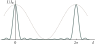
\includegraphics[scale=0.95]{figures/ch_17/fig_17_18.pdf}
		\caption[]{}
        % \caption[]{Plot of the function $I(\delta)$ for $N=10$. The principal maxima become narrower and narrower with an increase in the number of interfering rays. The secondary maxima are so weak that the interference pattern practically has the form of narrow bright lines on a dark background.}
		\label{fig:17_18}
	\end{center}
	\vspace{-0.85cm}
\end{figure}

Figure \ref{fig:17_18} shows a plot of the function $I(\delta)$ for $N=10$.
For comparison, a plot of the intensity for $N=2$ [two-beam interference; see the curve $I(x)$ in \fig{17_2}] is shown by a dash line.
Inspection of the figure shows that the principal maxima become narrower and narrower with an increase in the number of interfering rays.
The secondary maxima are so weak that the interference pattern practically has the form of narrow bright lines on a dark background.

Now, let us consider the interference of a very great number of rays whose intensity diminishes in a geometrical progression.
The oscillations being added have the form
\begin{equation}\label{eq:17_51}
    E_1 = a e^{i\omega t},\, E_2 = a \rho e^{i(\omega t+\delta)},\ldots, E_m = a \rho^{m-1} e^{i[\omega t+(m-1)\delta]}, \ldots,
\end{equation}

\noindent
($\rho$ is a constant quantity less than unity).
The resultant oscillation is described by the equation
\begin{equation*}
    E = \sum_{m=1}^N E_m = a e^{i\omega t} \sum_{m-1}^N \rho^{m-1} e^{i(m-1)\delta}.
\end{equation*}

\noindent
Using the expression for the sum of the terms of a geometrical progression, we get
\begin{equation*}
    E = a e^{i\omega t} \parenthesis{ \frac{1 - \rho e^{iN\delta}}{1 - \rho e^{i\delta}} } = \hat{A} e^{i\omega t}.
\end{equation*}

\noindent
Thus, the complex amplitude is
\begin{equation}\label{eq:17_52}
    \hat{A} = a \parenthesis{ \frac{1 - \rho e^{iN\delta}}{1 - \rho e^{i\delta}} }.
\end{equation}

If $N$ is very great, the complex number $\rho Ne^{iN\delta}$ may be disregarded in comparison with unity (we shall indicate as an example that $0.9^{100}\approx\num{4e-4}$).
Equation \eqref{eq:17_52} is thus simplified as follows:
\begin{equation*}
    \hat{A} = a \parenthesis{ \frac{1}{1 - \rho e^{i\delta}} }.
\end{equation*}

\noindent
Multiplying this equation by its complex conjugate, we get the square of the ordinary amplitude of the resultant oscillation:
\begin{align*}
    A^2 &= \hat{A}\hat{A}^* = \frac{a^2}{ \parenthesis{1 - \rho e^{i\delta}} \parenthesis{1 - \rho e^{-i\delta}} } = \frac{a^2}{ 1 + \rho^2 - \rho \parenthesis{e^{i\delta} + e^{-i\delta}} }\\
    &= \frac{a^2}{ 1 + \rho^2 - 2 \rho \cos\delta } = \frac{a^2}{ (1-\rho)^2 + 2\rho (1-\cos\delta) } \\
    &= \frac{a^2}{ (1-\rho^2) + 4\rho\sin^2(\delta/2) }.
\end{align*}

\noindent
Hence,
\begin{equation}\label{eq:17_53}
    I(\delta) = \frac{Ka^2}{(1-\rho^2) + 4\rho\sin^2(\delta/2)} = \frac{I_1}{(1-\rho^2) + 4\rho\sin^2(\delta/2)},
\end{equation}

\noindent
where $I_1=Ka^2$ is the intensity of the first (most intensive) ray.

At values of
\begin{equation}\label{eq:17_54}
    \delta = 2 \pi m \quad (m = 0, \pm 1, \pm 2, \ldots),
\end{equation}

\noindent
\eqn{17_53} has maxima equal to
\begin{equation}\label{eq:17_55}
    \ab{I}{max} = \frac{I_1}{(1-\rho)^2}.
\end{equation}

\noindent
In the intervals between maxima, the function changes monotonously, reaching a value equal to
\begin{equation}\label{eq:17_56}
    \ab{I}{min} = \frac{I_1}{(1-\rho)^2 + 4\rho} = \frac{I_1}{(1+\rho)^2}
\end{equation}

\noindent
at the middle of the interval.
Thus, the ratio of the intensity at a maximum to that at a minimum
\begin{equation}\label{eq:17_57}
    \frac{\ab{I}{max}}{\ab{I}{min}} = \parenthesis{\frac{1+\rho}{1-\rho}}^2
\end{equation}

\noindent
is the greater, the closer $\rho$ is to unity, \ie, the slower is the rate of diminishing of the intensity of the interfering rays.
Figure \ref{fig:17_19} shows a graph of function \eqref{eq:17_53} for $\rho=0.8$.
It can be seen from the figure that the interference pattern has the form of narrow sharp
lines on a virtually dark background.
Unlike \fig{17_18}, secondary maxima are absent.

\begin{figure}[t]
	\begin{center}
		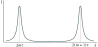
\includegraphics[scale=0.95]{figures/ch_17/fig_17_19.pdf}
		\caption[]{}
        % \caption[]{Graph of function \eqref{eq:17_53} for $\rho=0.8$. The interference pattern has the form of narrow sharp lines on a virtually dark background. Secondary maxima are absent.}
		\label{fig:17_19}
	\end{center}
	\vspace{-0.85cm}
\end{figure}

A practical case of a great number of rays with a diminishing intensity is encountered in the \textbf{Fabry-Perot interferometer}.
This instrument consists of two glass or quartz plates separated by an air gap (\fig{17_20}).
The internal surfaces of the plates are thoroughly polished so that the irregularities on them do not exceed several hundredths of the length of a light wave.
Next partly transparent metal layers or dielectric films\footnote{Metal layers have the shortcoming that they absorb light rays to a great extent. This is why recent years have seen their replacement with multilayer dielectric coatings having a high reflectivity.} are applied to these surfaces.
The outer surfaces of the plates are at a slight angle relative to the inner ones to eliminate the highlights due to the reflection of light from these surfaces.
In the original design of the interferometer, one of the plates could be moved relative to the other stationary one with the aid of a micrometric screw.
The unreliability of this design, however, resulted in its coming out of use.
In modern designs, the plates are secured rigidly.
The parallelity of the internal working planes is achieved by installing an invar or quartz ring\footnote{Both these materials are distinguished by their extremely low temperature
coefficient of expansion.} between the plates.
This ring has three projections with thoroughly polished edges at each side.
The plates are pressed against the ring by springs.
This design reliably ensures strict parallelity of the internal planes of the plates and constancy of the distance between them.
Such an interferometer with a fixed distance between its plates is known as a \textbf{Fabry-Perot etalon}.

\begin{figure}[t]
	\begin{minipage}[t]{0.38\linewidth}
		\begin{center}
			\includegraphics[scale=1]{figures/ch_17/fig_17_20.pdf}
			\caption[]{}
            % \caption[]{Scheme of a Fabry-Perot interferometer. It consists of two glass or quartz plates separated by an air gap. The internal surfaces of the plates are thoroughly polished so that the irregularities on them do not exceed several hundredths of the length of a light wave.}
			\label{fig:17_20}
		\end{center}
	\end{minipage}
	\hfill{ }%space{-0.05cm}
	\begin{minipage}[t]{0.62\linewidth}
		\begin{center}
			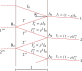
\includegraphics[scale=0.85]{figures/ch_17/fig_17_21.pdf}
            \caption[]{}
			% \caption[]{Ray entering the gap between the plates as described by \fig{17_20}. Interference in a Fabry-Perot interferometer.}
			\label{fig:17_21}
		\end{center}
	\end{minipage}
\vspace{-0.4cm}
\end{figure}

Let us see what happens to a ray entering the gap between the plates (\fig{17_21}).
Assume that the intensity of the entering ray is $I_0$.
At point A$_1$, this ray is divided into ray $1$ emerging outward and reflected ray $1'$.
If the coefficient of reflection from the surface of the plate is $\rho$, then the intensity of ray $1$ will be $I_1=(1-p)I_0$, and the intensity of the reflected ray will be $I_1'=\rho I_0$\footnote{We disregard the absorption of light in the reflecting layers and inside the plates.}.
At point B$_1$, ray $1'$ is divided into two.
Ray $1''$ shown by a dash line will drop out of consideration, while reflected ray $1''$ will have an intensity of $I_1''=\rho I_1'=\rho^2I_0$.
At point A$_2$, ray $1''$ will be divided into two rays---ray $2$ emerging outward having an intensity of $I_2=(1-\rho)I_1''=(1-\rho)\rho^2/I_0$ and reflected ray $2'$, and so on.
Thus, the following relation holds for the intensities of rays $1$, $2$, $3$, etc. emerging
from the instrument:
\begin{equation*}
    I_1 : I_2 : I_3 : \ldots = 1 : \rho^2 : \rho^4 : \ldots .
\end{equation*}

\noindent
Accordingly, for the amplitudes of the oscillations we have
\begin{equation*}
    A_1 : A_2 : A_3 : \ldots = 1 : \rho : \rho^2 : \ldots
\end{equation*}

\noindent
[compare with \eqn{17_51}].

The oscillation in each of the rays $2$, $3$, $4$, $\ldots$, lags in phase behind the oscillation in the preceding ray by the same amount $\delta$ determined by the optical path difference $\Delta$ appearing on the path A$_1$-B$_1$-A$_2$ or A$_2$-B$_2$-A$_3$, etc. (see \fig{17_21}).
A glance at the figure shows that $\Delta=2l/\cos\varphi$, where $\varphi$ is the angle of incidence of the rays on the reflecting layers.

If we gather rays $1$, $2$, $3$, $\ldots$, with the aid of a lens at point P of its focal plane (see \fig{17_20}), then the oscillations produced by these rays will have the form given by \eqn{17_51}.
Hence, the intensity at point P is determined by \eqn{17_53}, in which $\rho$ has the meaning of the coefficient of reflection, and
\begin{equation*}
    \delta = \frac{2\pi}{\lambda} = \frac{2l}{\cos\varphi}.
\end{equation*}

\begin{figure}[t]
	\begin{center}
		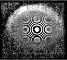
\includegraphics[scale=0.9]{figures/ch_17/fig_17_22.pdf}
		\caption[]{}
        % \caption[]{When a diverging beam of light is passed through the Fabry-Perot interferometer instrument, fringes of equal inclination having the form of sharp rings are produced in the focal plane of the lens.}
		\label{fig:17_22}
	\end{center}
	\vspace{-0.8cm}
\end{figure}

When a diverging beam of light is passed through the instrument, fringes of equal inclination having the form of sharp rings (\fig{17_22}) will be produced in the focal plane of the lens.

The Fabry-Perot interferometer is used in spectroscopy to study the fine structure of spectral lines.
It has also come into great favour in metrology for comparing the length of the standard metre with the wavelengths of individual spectral lines.
